\documentclass[a0,portrait,final]{a0poster}
% You might find the 'draft' option to a0 poster useful if you have
% lots of graphics, because they can take some time to process and
% display. (\documentclass[a0,draft]{a0poster})

% Switch off page numbers on a poster, obviously, and section numbers too.
\pagestyle{empty}
\setcounter{secnumdepth}{0}

% The textpos package is necessary to position textblocks at arbitary 
% places on the page.
\usepackage[absolute]{textpos}

% Graphics to include graphics. Times is nice on posters, but you
% might want to switch it off and go for CMR fonts.
\usepackage{graphics,wrapfig,times}

% These colours are tried and tested for titles and headers. Don't
% over use color!
\usepackage{color}
\definecolor{darkblue}{rgb}{0.1,0.1,0.5}
\definecolor{darkred}{rgb}{0.8,0.0,0.1}

% see documentation for a0poster class for the size options here
%\let\Textsize\normalsize
%\def\Head#1{\noindent\hbox to \hsize{\hfil{\LARGE\color{darkblue} #1}}\bigskip}
%\def\LHead#1{\noindent{\LARGE\color{darkblue} #1}\smallskip}
%\def\Subhead#1{\noindent{\large\color{darkblue} #1}}
%\def\Title#1{\noindent{\VeryHuge\color{darkred} #1}}

% Set up the grid
%
% Note that [40mm,40mm] is the margin round the edge of the page --
% it is _not_ the grid size. That is always defined as 
% PAGE_WIDTH/HGRID and PAGE_HEIGHT/VGRID. In this case we use
% 15 x 25. This gives us a wide central column for text (7 grid
% spacings) and two narrow columns (3 each) at each side for 
% pictures, separated by 1 grid spacing.
%
% Note however that texblocks can be positioned fractionally as well,
% so really any convenient grid size can be used.
%
\TPGrid[25mm,25mm]{15}{25}  % 3 - 1 - 7 - 1 - 3 Columns

% Mess with these as you like
\parindent=0pt
\parskip=1.0\baselineskip
%\renewcommand{\baselinestretch}{0.95}


%\usepackage{amsmath,amsthm, amssymb, latexsym}
\usepackage{fix-cm}
\usepackage[english]{babel}
\usepackage[latin1]{inputenc}
\usepackage{times}
\usepackage[T1]{fontenc}
\usepackage{calc} 
\usepackage[amssymb,thinspace]{SIunits}

% PGF includes
\usepackage{pgf,pgfplots}
\usepackage{tikz}
\usetikzlibrary{shadows,calc,plotmarks}
\usetikzlibrary{shapes,arrows,patterns}
\pgfdeclarelayer{background}
\pgfdeclarelayer{foreground}
\pgfsetlayers{background,main,foreground}
%\usetikzlibrary{,decorations,backgrounds,matrix,automata,trees,shapes,}

%%%%%
\newcommand{\posterheading}[1]{
	\begin{center}
	  \begin{tikzpicture}
		\definecolor{darkblue}{rgb}{0.1,0.5,0.1}
		\node [draw=none,rounded corners=0.5ex, 
			minimum height=5ex, minimum width=0.95\columnwidth, 
			top color= darkblue!60, bottom color= darkblue!90]
			%top color= black!40, bottom color=black!70]
			{
				\color{white}{\huge #1}
			};
	  \end{tikzpicture}
	\end{center}
}

\newcommand{\postertitle}[3]{
	\begin{center}
	  \begin{tikzpicture}
		\definecolor{darkblue}{rgb}{0.1,0.1,0.5}
		\node [draw=none,rounded corners=3ex, 
			minimum height=40ex, minimum width=\columnwidth]
			{
				\begin{tabular}{c}
				\color{black}{\bf \veryHuge #1}\\ \\
				\color{darkblue}{\Huge #2}\\ \\
				\color{darkblue}{\LARGE {#3}}\\
				\end{tabular}
			};
	  \end{tikzpicture}
	\end{center}
}

\newcommand{\alert}[1]{{\color{darkred}{#1}}}
\renewcommand{\normalsize}{\Large}
%%%%%

%-------------------------------------------------------------------------
%-------------------------------------------------------------------------
\begin{document}


%-------------------------------------------------------------------------
% Header
%-------------------------------------------------------------------------
\begin{textblock}{15}(0,-1)
\postertitle
{\begin{tabular}{c}
Integrating Learning into a BDI Agent for Environments\\ with Changing Dynamics
\end{tabular}}
{Dhirendra~Singh$^1$~~~
Sebastian~Sardina$^1$~~~
Lin~Padgham$^1$~~~
Geoff~James$^2$}
{\begin{tabular}{c}
	$^1$RMIT University, Melbourne, Australia\\
	$^2$CSIRO Energy Technology, Sydney, Australia
\end{tabular}}
\end{textblock}


%-------------------------------------------------------------------------
% Summary
%-------------------------------------------------------------------------
\begin{textblock}{4.6}(0.2,3.75)
\posterheading{Summary}
This paper extends our earlier work integrating \alert{learning to improve plan selection} in the popular Belief, Desire, Intentions (BDI) agent paradigm.

Here we address the problem that learning in deployed agents must be \alert{continuous} rather than a one-off process.

Our main contribution is a novel confidence measure which allows the agent to \alert{adjust its reliance on the learning dynamically}, facilitating in principle infinitely many (re)learning phases. 

We demonstrate the benefits of the approach in an example battery controller for energy management.

\begin{center}
	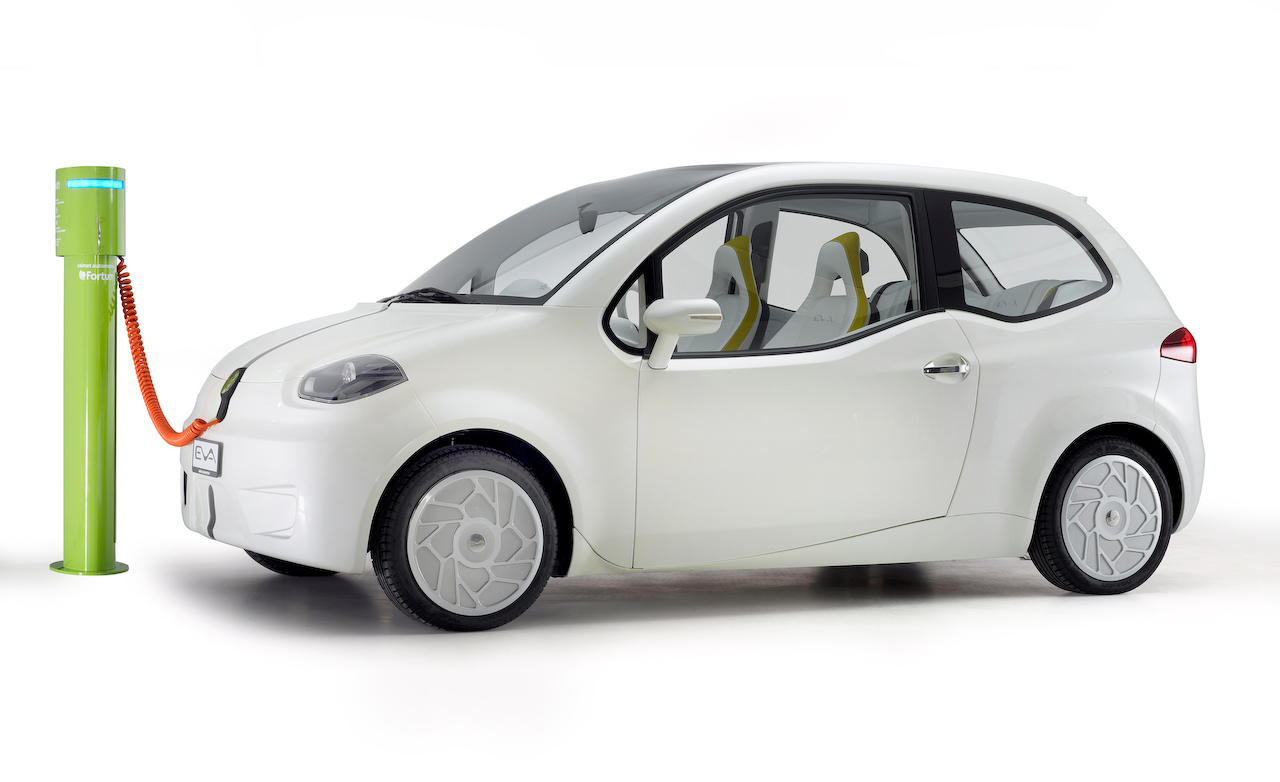
\includegraphics[width=0.9\columnwidth]{figs/valmet-eva-electric-car-concept-11.jpg}
\end{center}


\end{textblock}

%-------------------------------------------------------------------------
% BDI Architecture
%-------------------------------------------------------------------------
\begin{textblock}{4.6}(0.2,13)
\posterheading{BDI Architecture}

A \alert{plan} is a rule $e: \psi \leftarrow \delta$; program $\delta$ is a strategy for goal $e$ when \alert{context condition $\psi$} holds.

Plans may perform primitive actions or post sub-goals that are handled in a \alert{hierarchical} manner.

\begin{center}
%!TEX root = ../dsingh-aamas10-poster.tex
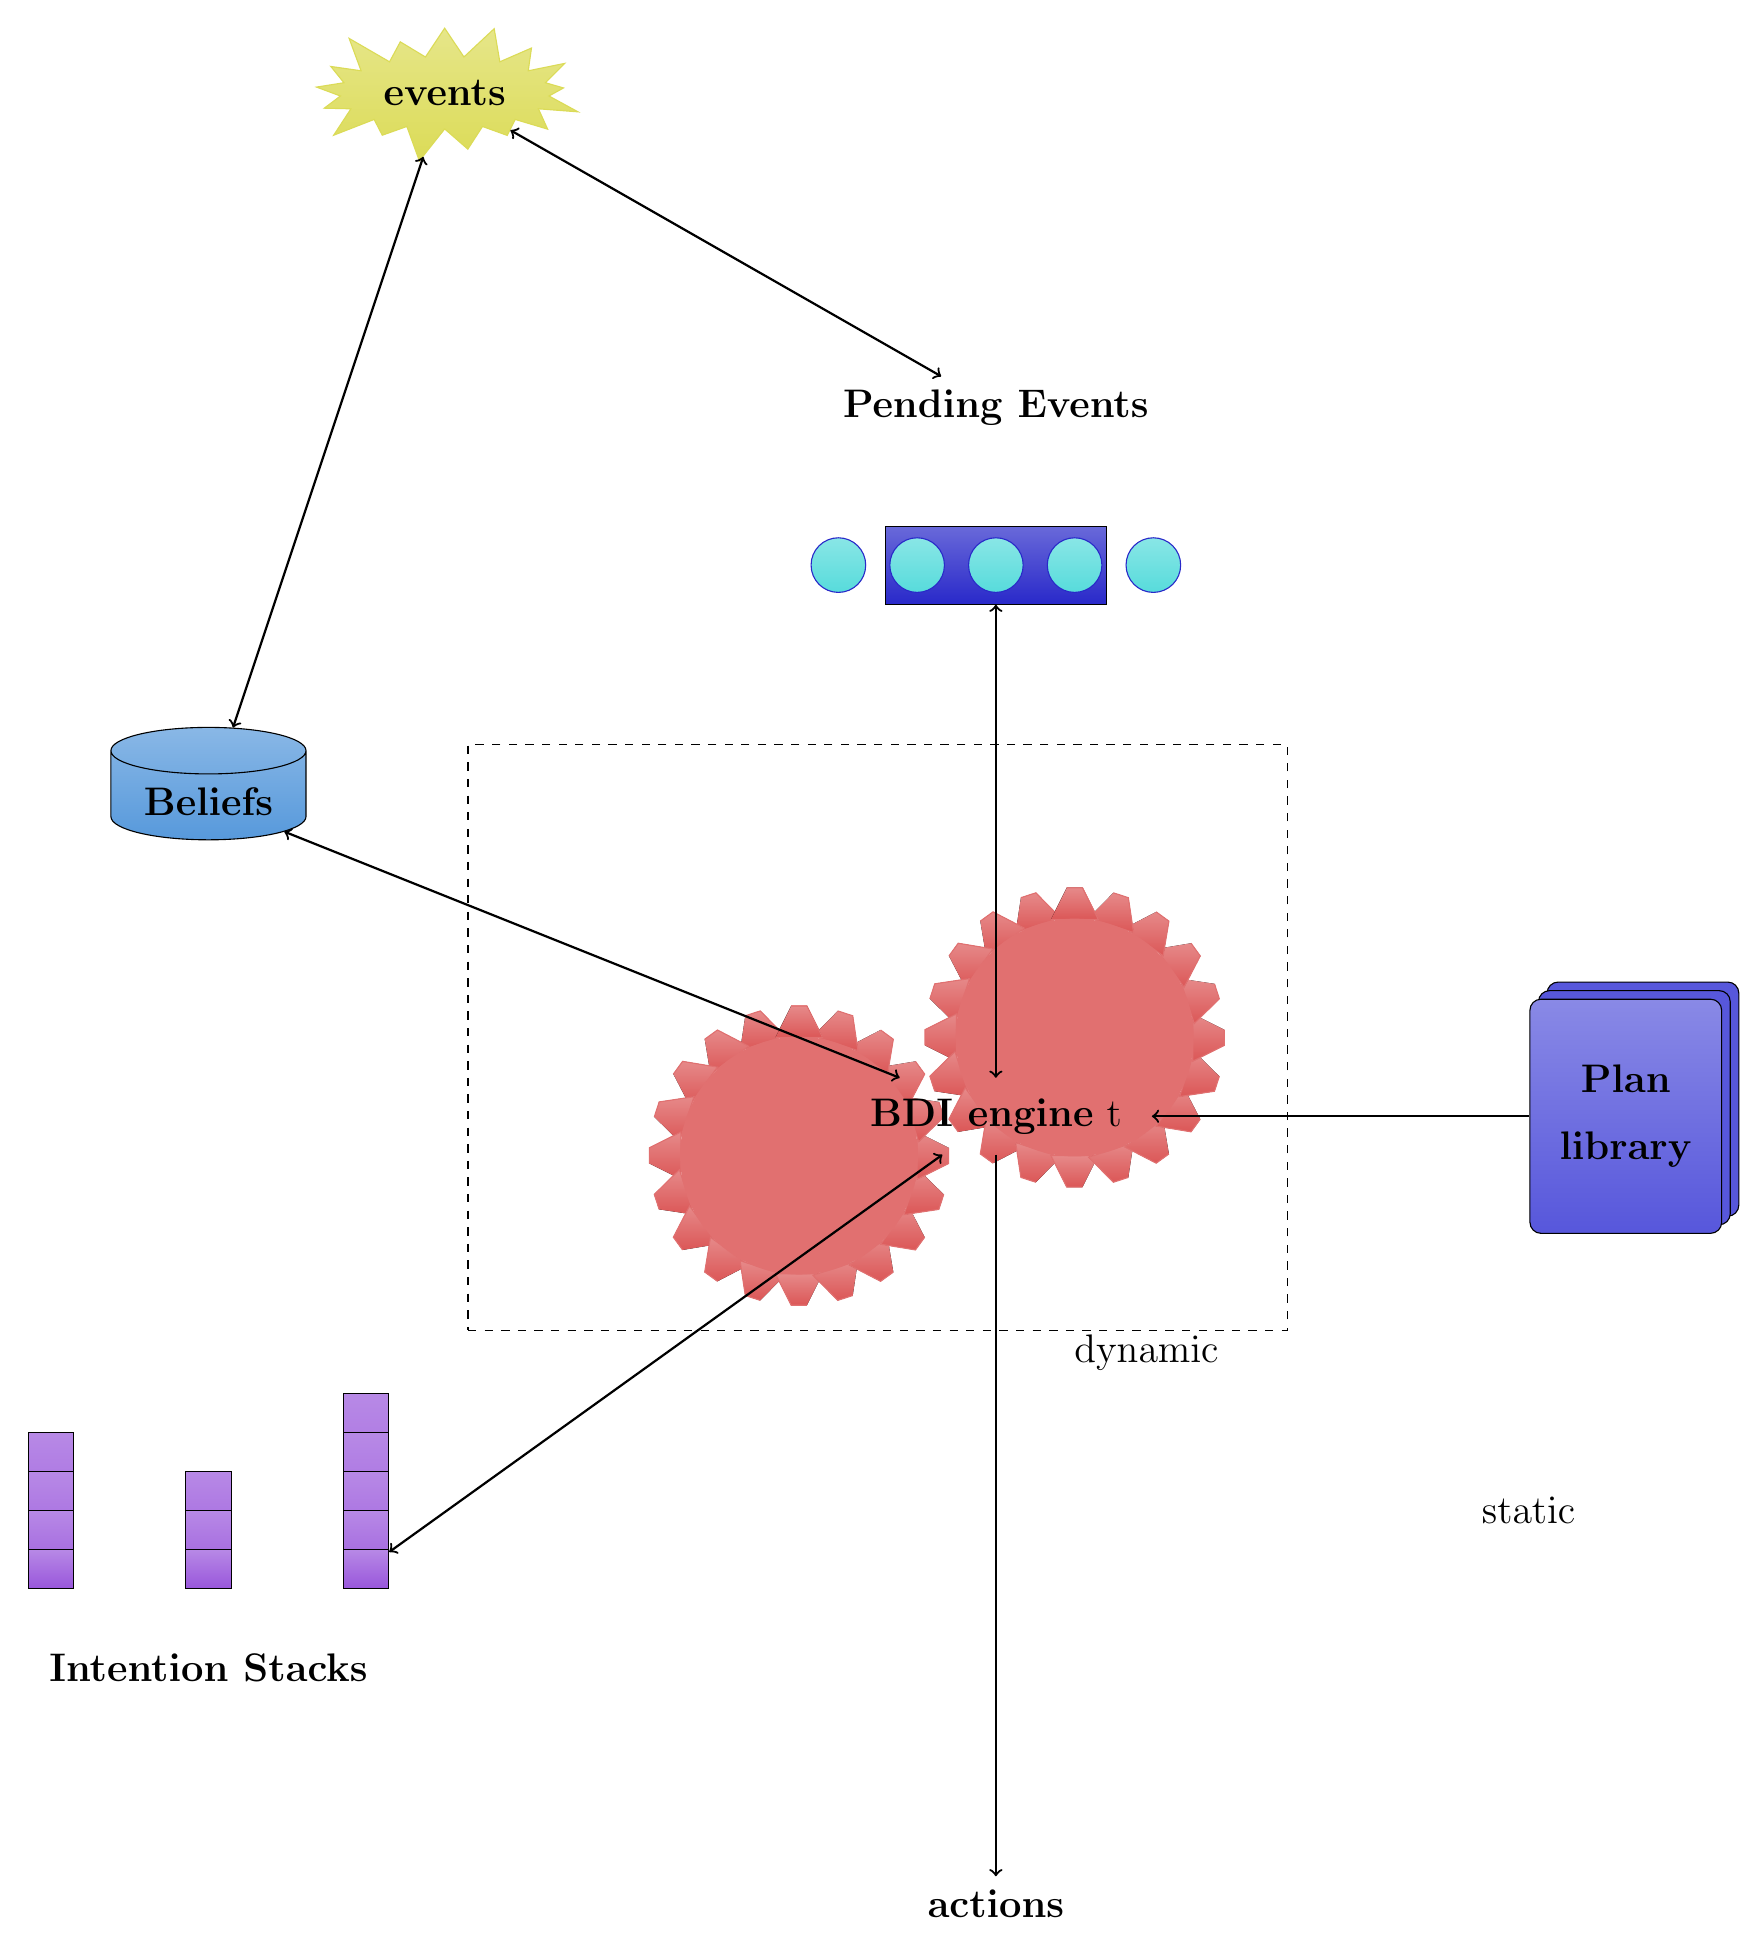
\begin{tikzpicture}

\definecolor{green1}{rgb}{0.86,0.86,0.34}
\definecolor{red1}{rgb}{0.86,0.34,0.34}
\definecolor{blue5}{rgb}{0.6,0.34,0.86}
\definecolor{blue4}{rgb}{0.16,0.16,0.79}
\definecolor{blue3}{rgb}{0.34,0.86,0.86}
\definecolor{blue2}{rgb}{0.34,0.6,0.86}
\definecolor{blue1}{rgb}{0.34,0.34,0.86}

\tikzstyle{centityd}=[draw=black]
\tikzstyle{centityf}=[fill=blue1!30]
\tikzstyle{centity}=[centityd,centityf]
\tikzstyle{entity}=[centity,thick,text centered,anchor=center]



%%% Beliefs
\node (database) at (-3,10)  (B)
	[draw=black,top color=blue2!70, bottom color=blue2,cylinder,shape border rotate=90,minimum width=5em,shape aspect=.3]
	{\textbf{Beliefs}};


%%% Pending Events
\node at (7,15) (eventQueue) {{\bf Pending Events}};
\begin{pgfonlayer}{foreground}
\foreach \x in {5,6,...,9}
\draw [draw=blue4,top color=blue3!70, bottom color=blue3](\x,13) circle (.7em);
\end{pgfonlayer}
\draw (7,13) node (Q) 
	[draw=black,top color=blue4!70, bottom color=blue4,text width=5em, minimum height=2em] {};

%%% Plan Library
\node at (15,6)(P) 
	[draw=black,top color=blue1!70, bottom color=blue1,
	rounded corners, double copy
	shadow={fill=blue1},text centered, 
	minimum height=6em] 
	{	\begin{tabular}{c} 
          \textbf{Plan} \\[1ex]
          \textbf{library}
         \end{tabular}	};
\node[anchor=west] at (13,1) {static};

%%% Intention Stacks
\foreach \x in {4,3,2,1}
\draw (-5,0) node (I) [anchor=south,draw=black,top color=blue5!70, bottom color=blue5,text width=0.5em,
	minimum height=\x em]{};
\foreach \x in {3,2,1}
\draw (-3,0) node (I) [anchor=south,draw=black,top color=blue5!70, bottom color=blue5,text width=0.5em,
	minimum height=\x em]{};
\foreach \x in {5,4,3,2,1}
\draw (-1,0) node (I) [anchor=south,draw=black,top color=blue5!70, bottom color=blue5,text width=0.5em,
	minimum height=\x em]{};
\node at (-3,-1) (Intentions) {{\bf  Intention Stacks}};

%%% BDI Engine
\foreach \x in {0,18,...,360}
\fill [rotate around={\x:(4.5,5.5)}, draw=red1!85, top color=red1!70,bottom color=red1] 
	(4.2,7.0) -- (4.8,7.0) -- (4.6,7.4) -- (4.4,7.4);
\fill [fill=red1!85] (4.5,5.5) circle (1.51);

\foreach \x in {0,18,...,360}
\fill [rotate around={\x:(8.0,7.0)}, draw=red1!85, top color=red1!70,bottom color=red1] 
	(7.7,8.5) -- (8.3,8.5) -- (8.1,8.9) -- (7.9,8.9);
\fill [fill=red1!85] (8.0,7.0) circle (1.51);

\node[anchor=east] at (10,3)  {dynamic};

%%% Events
\node at (0,19) [starburst,draw=green1,top color=green1!70, bottom color=green1] (in) {{\bf events}};

%%% Labels and Arrows
\begin{pgfonlayer}{foreground}
\node[anchor=center] at (7,6)  (deli) 
	{\begin{tabular}{c}
     	\textbf{BDI engine} t
     \end{tabular}};
\node at (7,-4) (actions) {{\bf actions}};
\draw[thick,->] (deli) -- (actions) ; 
\draw[thick,<->] (deli) -- (I) ; 
\draw[thick,<->] (deli) -- (B) ; 
\draw[thick,<-] (deli) -- (P) ;
\draw[thick,<->] (deli) -- (Q) ; 
\draw[thick,<->] (in) -- (eventQueue) ; 
\draw[thick,<->] (in) -- (B) ; 
\end{pgfonlayer}

%%% Encapuslating box
\begin{pgfonlayer}{background}
\node[draw,dashed,rectangle,minimum height=15em,minimum width=21em ] at (5.5,7){};
\end{pgfonlayer}


\end{tikzpicture}
\end{center}

Traditionally, \alert{BDI agents have no learning ability}, and cannot adjust to changes that cause previously successful approaches to fail.

\end{textblock}


%-------------------------------------------------------------------------
% BDI Learning Framework
%-------------------------------------------------------------------------
\begin{textblock}{4.6}(5.2,3.75)
\posterheading{BDI Learning Framework}

Our learning framework augments plan's context conditions with \alert{decision trees}, allowing \alert{plan applicability} to be learnt from experience.

Using a \alert{probabilistic plan selection} function, the agent balances exploration and exploitation of plans.

\begin{center}

\begin{tikzpicture}[>=latex]
\definecolor{brown3}{rgb}{0.86,0.6,0.34}
	\node [text width=12em, draw=brown3, 
	top color=brown3!70, bottom color=brown3] at (0,0) (A) {
		Record outcomes for chosen plans to train decision trees
	};
	\node [text width=12em, draw=brown3, 
	top color=brown3!70, bottom color=brown3] at (0,-6) (B) {
		Probablistically select plans based on ongoing learning
		};
	\draw[brown3,] (-9,0) edge[out=210,in=150,line width=50,]  (-9,-6);
	\draw[brown3] (9,0) edge[out=330,in=30,line width=50]  (9,-6);
\end{tikzpicture}
\end{center}
\alert{Acting and learning are interleaved} in an \alert{online} manner, i.e.,  current learning influences ongoing choices that impact subsequent learning.

\end{textblock}

%-------------------------------------------------------------------------
% Confidence in Learning
%-------------------------------------------------------------------------
\begin{textblock}{4.6}(5.2,11.75)
\posterheading{Confidence in Learning}

We \alert{build confidence from observed performance} of a plan by evaluating
how well-informed were the recent decisions, or \alert{stability-based} measure, and how well we know the worlds we are witnessing, or \alert{world-based} measure.


Plan selection weight, that dictates \alert{exploration}, is then calculated using the predicted \alert{likelihood of success} and the dynamic \alert{confidence} measure.

\begin{center}
%!TEX root = ../dsingh-ijcai11-poster.tex
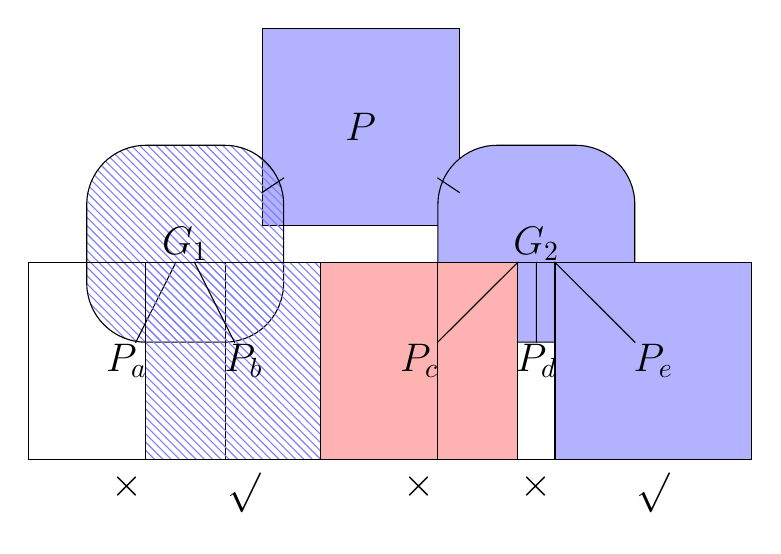
\begin{tikzpicture}[level distance=3em]
\tikzstyle{succ}=[label=below:$\surd$]
\tikzstyle{fail}=[label=below:$\times$]
\tikzstyle{trace}=[solid,style=circle,fill=black!20,above left=0.15cm,scale=.7]

\tikzstyle{planbox}=[draw,minimum height=2.5cm,minimum width=2.5cm]
\tikzstyle{goalbox}=[draw,minimum height=2.5cm,minimum width=2.5cm,rounded corners=0.75cm]
\tikzstyle{planbox2}=[planbox,pattern=north west lines,pattern color=blue!50]
\tikzstyle{goalbox2}=[goalbox,pattern=north west lines,pattern color=blue!50]
\tikzstyle{goalbox3}=[goalbox,fill=blue!30]
\tikzstyle{planbox3}=[planbox,fill=blue!30]
\tikzstyle{planbox4}=[planbox,fill=red!30]

\tikzstyle{level 1}=[sibling distance=9em] 
\tikzstyle{level 2}=[sibling distance=3em] 

\node[planbox3,solid] {$P$}
				child[solid] {node[goalbox2] {$G_{1}$}
					child {node[planbox,fail] {$P_{a}$}}
					child {node[planbox2,succ] {$P_{b}$}}
				}
				child[solid] {node[goalbox3] {$G_{2}$}
					child {node[planbox4,fail] {$P_{c}$}}
					child {node[planbox,fail] {$P_{d}$}}
					child {node[planbox3,succ] {$P_{e}$}}
				}

;

\end{tikzpicture}

\end{center}

\alert{Example}: Say plan $P_c$ no longer works for resolving goal $G_2$ after execution $15$, and plan $P_e$ does instead.
As plan $P_c$ starts to fail, the perceived confidence ($y$-axis) drops, \alert{promoting new exploration} and (re)learning.

\begin{center}
%!TEX root = ../dsingh-ijcai11-talk.tex
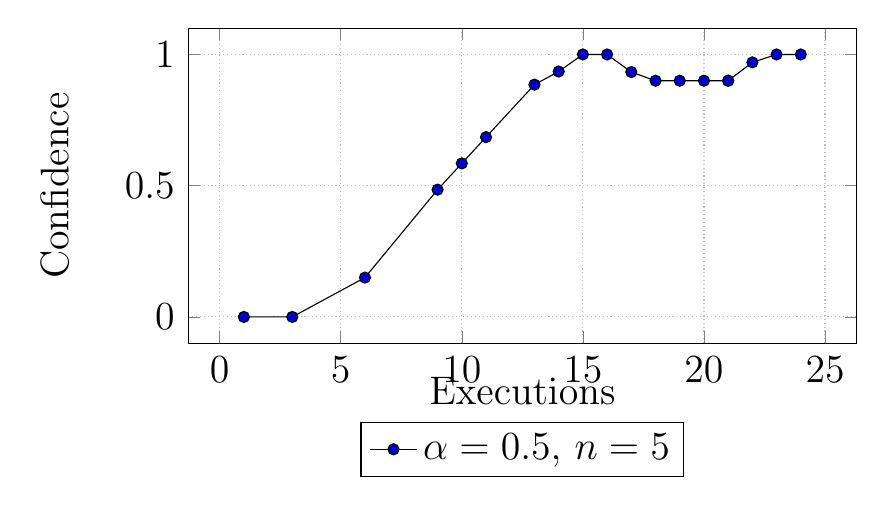
\begin{tikzpicture}

\begin{axis}[
width=0.7\columnwidth,height=4cm,scale only axis,
axis line style={-}, xtick style={-}, ytick style={-},
ymin=0,ymax=1, enlarge y limits=true,
xlabel=Executions,
ylabel=Confidence,
every axis y label/.style={at={(-0.2,0.5)},rotate=90,anchor=center}, 
every axis x label/.style={at={(0.5,-0.15)},anchor=center},
grid=both,grid style={-,style=densely dotted},
%legend style={at={(0.7,0.25)},anchor=north west},
legend style={at={(0.5,-0.25)}, anchor=north,legend columns=-1},
%cycle list name=black white,
] 

% alpha=0.5
\addplot+[black] coordinates { 
	(1,0.000) (3,0.000) (6,0.150) (9,0.485) (10,0.585) 
	(11,0.685) (13,0.885) (14,0.935) (15,1.000) (16,1.000) 
	(17,0.933) (18,0.900) (19,0.900) (20,0.900) (21,0.900) 
	(21,0.900) (22,0.970) (23,1.000) (24,1.000) 
};
\addlegendentry{$\alpha=0.5$, $n=5$}

\end{axis} 
\end{tikzpicture} 

\end{center}

\end{textblock}

%-------------------------------------------------------------------------
% Modular Battery Controller
%-------------------------------------------------------------------------
\begin{textblock}{4.6}(10.2,3.75)
\posterheading{Modular Battery Controller}

%\begin{wrapfigure}{l}{1.1\columnwidth}
\begin{center}
\vskip -1.0em
	
\includegraphics[width=0.9\columnwidth]{figs/smart-home.jpg}
\end{center}
%\end{wrapfigure}
A building with local generation and loads is to restrict power consumption to a set range, using a modular battery system that can be charged or discharged as needed. 

A \alert{programmed solution is not ideal} since battery performance is susceptible to change over time.
 
We design a \alert{learning BDI controller} that works to initial specification but also \alert{adapts} to ongoing changes in the battery system.

\alert{Scenario 1}: Recovery from deterioration in module capacities at $5\kilo$ episodes.
\begin{center}
%!TEX root = ../dsingh-ijcai11-poster.tex
\begin{tikzpicture}
\definecolor{darkred}{rgb}{0.8,0.0,0.1}
\definecolor{darkblue}{rgb}{0.1,0.1,0.5}

\begin{axis}[
width=0.75\columnwidth,height=8cm,scale only axis,
axis line style={-}, xtick style={-}, ytick style={-},
%xlabel=Episodes,
%ylabel=Success,
%every axis y label/.style={at={(-0.12,0.5)},rotate=90,anchor=center}, 
%every axis x label/.style={at={(0.5,-0.15)},anchor=center},
grid=both,grid style={-,style=densely dotted},
legend style={at={(0.5,0.25)},anchor=north west},
scaled x ticks = false,
xtick={0,5e3,10e3,15e3,20e3,25e3,30e3,35e3,40e3},
xticklabels={$0$,$5\kilo$,$10\kilo$,$15\kilo$,$20\kilo$,$25\kilo$,$30\kilo$,$35\kilo$,$40\kilo$}
] 

\addplot[darkblue,-,line width=2pt] file {./data/storage1b.CF.tikzdata};
%\addlegendentry{Data} 

\end{axis} 
\end{tikzpicture} 

\end{center}
\vskip -1.0em
\alert{Scenario 2}: Recovery from individual module failures during $[0,20\kilo]$, $[20\kilo,40\kilo]$ episodes.
\begin{center}
%!TEX root = ../dsingh-ijcai11-poster.tex
\begin{tikzpicture}
\definecolor{darkred}{rgb}{0.8,0.0,0.1}
\definecolor{darkblue}{rgb}{0.1,0.1,0.5}

\begin{axis}[
width=0.75\columnwidth,height=8cm,scale only axis,
axis line style={-}, xtick style={-}, ytick style={-},
%xlabel=Episodes,
%ylabel=Success,
%every axis y label/.style={at={(-0.12,0.5)},rotate=90,anchor=center}, 
%every axis x label/.style={at={(0.5,-0.15)},anchor=center},
grid=both,grid style={-,style=densely dotted},
legend style={at={(0.5,0.25)},anchor=north west},
scaled x ticks = false,
xtick={0,5e3,10e3,15e3,20e3,25e3,30e3,35e3,40e3},
xticklabels={$0$,,$10\kilo$,,$20\kilo$,,$30\kilo$,,$40\kilo$}
] 

\addplot[darkblue,-,line width=2pt] file {./data/storage2b.CF.tikzdata};
%\addlegendentry{Data} 

\end{axis} 
\end{tikzpicture} 

\end{center}
\vskip -1.0em
\alert{Scenario 3}: Recovery from complete system failure during $[0,5\kilo]$ episodes.
\begin{center}
%!TEX root = ../dsingh-ijcai11-poster.tex
\begin{tikzpicture}
\definecolor{darkred}{rgb}{0.8,0.0,0.1}
\definecolor{darkblue}{rgb}{0.1,0.1,0.5}

\begin{axis}[
width=0.75\columnwidth,height=8cm,scale only axis,
axis line style={-}, xtick style={-}, ytick style={-},
%xlabel=Episodes,
%ylabel=Success,
%every axis y label/.style={at={(-0.12,0.5)},rotate=90,anchor=center}, 
%every axis x label/.style={at={(0.5,-0.15)},anchor=center},
grid=both,grid style={-,style=densely dotted},
legend style={at={(0.5,0.25)},anchor=north west},
scaled x ticks = false,
xtick={0,5e3,10e3,15e3,20e3,25e3,30e3,35e3,40e3},
xticklabels={$0$,$5\kilo$,$10\kilo$,$15\kilo$,$20\kilo$,$25\kilo$,$30\kilo$,$35\kilo$,$40\kilo$}
] 

\addplot[darkblue,-,line width=2pt] file {./data/storage3mb.CF.tikzdata};
%\addlegendentry{Data} 

\end{axis} 
\end{tikzpicture} 

\end{center}

The above experiments plot average success in configuring the battery correctly ($y$-axis) over the number of episodes ($x$-axis) for various changes in the environment dynamics. 

\end{textblock}


%-------------------------------------------------------------------------
% Footer
%-------------------------------------------------------------------------
\begin{textblock}{15}(0,24)
\begin{center}
\color{darkred}{\LARGE
D.~Singh, S.~Sardina, L.~Padgham, G.~James, Integrating Learning into a {BDI} Agent for Environments with Changing Dynamics. In {\it Proceedings of International Joint Conference on Artificial Intelligence (IJCAI)}, Barcelona, Spain, 2011.
}
\end{center}
\end{textblock}


%-------------------------------------------------------------------------
%-------------------------------------------------------------------------
\end{document}